\documentclass[runningheads]{llncs}
\usepackage{graphicx}
\usepackage{booktabs}
\usepackage{multirow}
\usepackage{amsmath}
\usepackage{amssymb}
\usepackage{hyperref}

\begin{document}

\title{Domain-Aware Tuberculosis Screening with a Single LoRA-Adapted CXR Foundation Model}

\titlerunning{Domain-Aware TB Screening with a LoRA-Adapted Foundation Model}

\author{Eunchan Hwang}
\authorrunning{E. Hwang}
\institute{MI2RL}

{\LARGE\bfseries Domain-Aware Tuberculosis Screening with a Single LoRA-Adapted CXR Foundation Model\par}
\vspace{0.5em}
{\large Eunchan Hwang\par}
{\itshape MI2RL\par}
\vspace{1em}

\maketitle

\begin{abstract}
Tuberculosis (TB) still kills more people each year than any other single
infectious disease, and automated chest X-ray (CXR) screening is one of the
few ways to scale diagnosis where radiologists are scarce [2]. We
build a TB/Normal classifier around a single frozen, self-supervised CXR
foundation model -- RAD-DINO [3] -- adapted with low-rank
adaptation (LoRA) [6] instead of full fine-tuning, and validated
with leave-one-imaging-modality-out (LOMO) cross-validation, the correct
proxy for cross-domain generalization once a real acquisition-domain signal
(\texttt{Modality\_DICOM}) sits inside the training pool. Our central
finding is negative and, we argue, more useful than another internal
score: on true external validation across three public cohorts, every
addition we made on top of this single backbone -- a second foundation
model, mask supervision, dual-stream fusion, and domain-aware mixup -- made
cross-institution performance \emph{worse}, not better, while improving or
barely changing the internal number. A component-wise ablation of the
domain-generalization machinery itself shows that strong image-level
augmentation carries essentially all of the benefit, and that removing
batch-level domain-aware mixup improves external F1. The resulting model --
one LoRA-adapted RAD-DINO, lung-cropped input, strong augmentation, no
mixup -- reaches F1@0.5 of 0.9913 internally and 0.8966 / 0.8976 on the
external Shenzhen and Montgomery cohorts (accuracy@0.5 0.8958 / 0.9058),
reaching for the first time the 89\% Shenzhen-accuracy bar of our earlier
DenseNet-121 baseline [1] while using a strictly simpler pipeline
than the ensemble it replaces.
\keywords{Tuberculosis screening \and Chest X-ray \and Foundation models \and Domain generalization \and LoRA}
\end{abstract}

\section{Introduction}

CXR classifiers routinely reach near-perfect accuracy on a held-out split
from their own training hospital, then fail on a different hospital,
scanner, or country. We saw this ourselves: a plain DenseNet-121, trained
without any domain-generalization (DG) technique, scored only 66\% accuracy
on the external Shenzhen cohort in our earlier work [1], rising to
89\% once MixStyle [7] and multi-level augmentation were added.
Fig.~\ref{fig:shortcut} shows why: Grad-CAM on that un-augmented baseline
fixates on a corner marker rather than any lung structure, for both a TB
case and a Normal case, despite a high score on a plain stratified split.
The model was not reading the X-ray -- it was reading a sticker.

\begin{figure}[t]
\centering
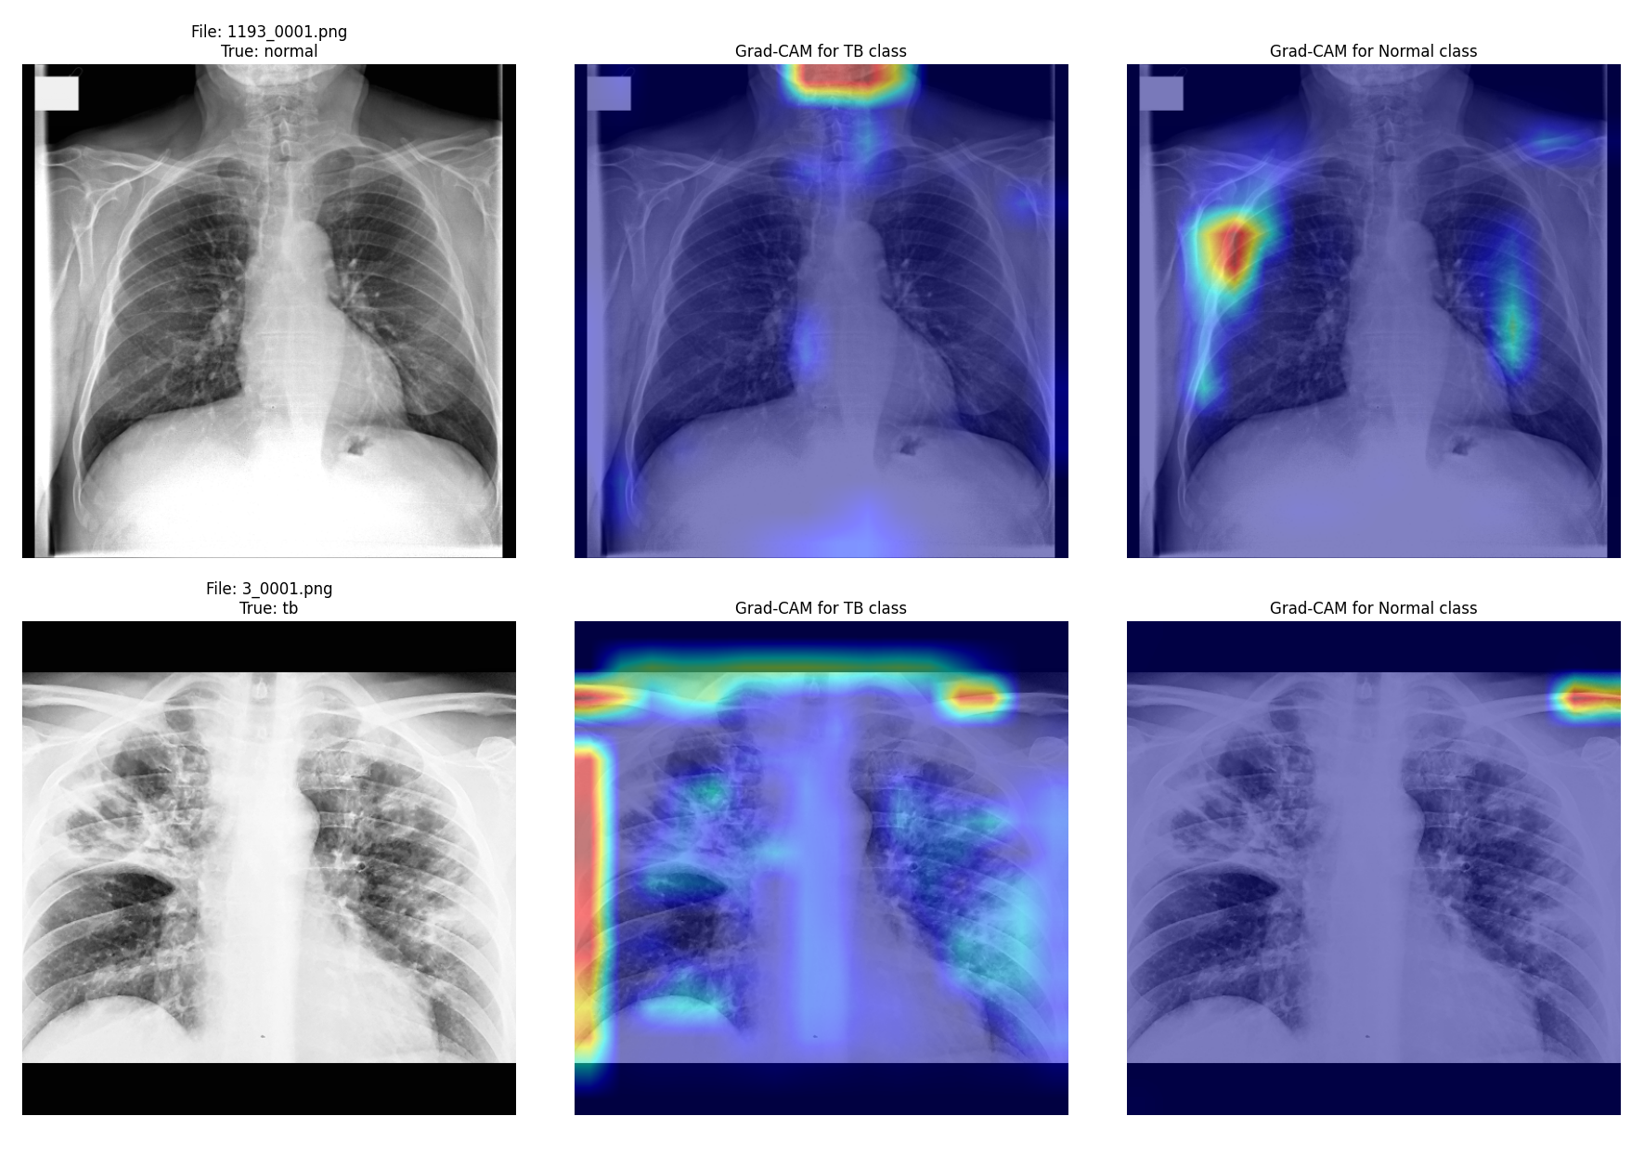
\includegraphics[width=0.92\textwidth]{fig1_shortcut_learning.png}
\caption{Grad-CAM on the un-augmented baseline, for a Normal case (top) and
a TB case (bottom). Both classes' attention fixates on a corner
marker/border artifact, not lung anatomy -- a shortcut a plain stratified
split rewards even though it carries no diagnostic signal.}
\label{fig:shortcut}
\end{figure}

This paper extends that recipe two ways. First, we replace the single
DenseNet-121 with a CXR-domain foundation model, RAD-DINO, frozen and
adapted with LoRA rather than fully fine-tuned -- cheaper to train and, we
find, harder for the model to overfit through. Second, we
validate with leave-one-modality-out (LOMO) cross-validation rather than a
plain stratified split: since \texttt{Modality\_DICOM} is itself a domain
signal present in the training data, a stratified split lets the model see
every modality during training and rewards exploiting exactly the kind of
shortcut Fig.~\ref{fig:shortcut} shows. LOMO instead holds out one whole
modality per fold, so a fold's validation score reflects generalization to
an acquisition setting the model never saw -- a much closer proxy for the
external-hospital deployment this system is actually meant for.

The third contribution is the one we consider most transferable. Having
measured every variant on three genuinely external cohorts rather than on
the internal split alone, we found that the usual direction of progress --
add a second foundation model, add anatomical supervision, add a
batch-level DG technique -- reliably improved the internal number while
degrading external performance. We therefore report a deliberately
subtractive result: the model we recommend is the smallest configuration
we tested, and each component we removed was removed because an ablation
showed it was not earning its complexity on data from a hospital the model
had never seen.

\section{Method}

\begin{figure}[t]
\centering
\fbox{\parbox[c][3.0cm][c]{0.92\textwidth}{\centering\itshape
[Architecture diagram: raw CXR $\to$ lung-crop $\to$ CLAHE $\to$ RAD-DINO
(frozen + LoRA) $\to$ 4-fold LOMO checkpoint averaging $\to$ decision at
$\tau=0.5$. See \texttt{diagram\_prompt.md}.]}}
\caption{Overview of the inference pipeline (placeholder -- see
\texttt{diagram\_prompt.md}).}
\label{fig:arch}
\end{figure}

\subsection{Backbones}

Our final model uses \textbf{RAD-DINO alone}. The remaining four encoders
below were trained and evaluated as comparisons, and are reported here
because the comparison is what justifies the choice -- not because any of
them is part of the recommended pipeline. We train and compare five
encoders: DenseNet-121 [10] (full
fine-tune, our prior baseline architecture), Swin-Tiny [11] and
ConvNeXt-Tiny [12] (added for architectural diversity at
negligible extra cost, both ImageNet-pretrained at 224px), and two
foundation models, each frozen and adapted with LoRA (rank 16, alpha 16, on
the attention/MLP linear layers):

\begin{itemize}
\item \textbf{RAD-DINO} [3]: a DINOv2 [5] ViT-B/14
  pretrained self-supervised on chest radiographs, 518px input.
\item \textbf{CheXFound} [4]: a DINOv2 ViT-L/16 pretrained on a
  large CXR corpus, 512px input, register tokens, SwiGLU feed-forward.
\end{itemize}

All five share one lightweight head: LayerNorm, Dropout, then a single
Linear layer over the pooled features.

\subsection{Preprocessing and domain generalization}

Every image is lung-cropped by a PSPNet segmenter [13]
before classification, CLAHE-normalized, and clipped to its 1st/99th
percentile intensity range. The final model then applies DG at exactly one
level, extending [1]:

\begin{itemize}
\item \textbf{Image-level (retained)}: the multi-level augmentation of
  [1], plus RandConv [8] (a freshly re-initialized
  random convolution, blended with the original image, that scrambles
  texture while roughly preserving shape), amplitude-spectrum perturbation
  (perturbing the Fourier amplitude, where scanner/contrast differences
  mostly live, while leaving the anatomy-carrying phase spectrum
  untouched), and resolution jitter, affine, colour-jitter and blur
  transforms stacked on top.
\end{itemize}

Two further DG components were implemented, evaluated, and then
\emph{removed} from the final model:

\begin{itemize}
\item \textbf{Batch-level, removed}: domain-aware mixup [9] pairs
  each sample with a partner from a \emph{different}
  \texttt{Modality\_DICOM} value and blends both images and labels, so
  synthesized samples interpolate along the domain axis this dataset
  actually has. Sect.~\ref{sec:dgablation} shows it does not help here:
  removing it improves external F1 on both Shenzhen and Montgomery, and
  mixup applied \emph{without} image-level augmentation is the worst of all
  seven configurations we tested. We attribute this to the fact that the
  four \texttt{Modality\_DICOM} values are acquisition tags on the same
  imaging type rather than genuinely distinct modalities, so the invariance
  mixup enforces is nearly orthogonal to the inter-hospital shift that
  actually costs us performance -- while the blended images themselves are
  anatomically impossible superpositions of two ribcages carrying a soft
  label with no test-time counterpart.
\item \textbf{Feature-level, not applicable}: MixStyle [7] mixes
  low-level style statistics across a mini-batch, but is wired into the
  DenseNet-121 path only -- the one backbone whose intermediate feature
  maps are cleanly hookable at the early layer MixStyle expects. Since the
  final model is RAD-DINO alone, MixStyle plays no part in it.
\end{itemize}

\texttt{Modality\_DICOM} itself never enters the model as an input feature
-- it is only ever a domain label for the DG techniques and the LOMO split,
never a shortcut for the classifier to key on.

\subsection{Training and validation protocol}

For each of the five encoders, we hold out one of the four imaging
modalities in the training pool (CR, DX, XA, XC) and train on the remaining
three, for 15 epochs per fold, repeating for all four modalities. This
measures generalization to an unseen acquisition modality directly; a
stratified split cannot, since it lets the model train on every modality
and rewards \texttt{Modality\_DICOM}-correlated shortcuts. At inference,
the four fold checkpoints are averaged into an implicit 4-way sub-ensemble
(the only form of ensembling the final model retains); where encoder
combinations are reported for comparison, they are averaged the same way.
The final configuration is therefore: RAD-DINO, LoRA rank 16, lung-cropped
input, LOMO folds, strong image-level augmentation, no mixup, 15 epochs per
fold, decision threshold fixed a priori at 0.5.

\section{Experiments}

\subsection{Data}
\label{sec:data}

Training and internal-validation data comes from the challenge's own
TB/Normal pool across four modalities (CR, DX, XA, XC). For genuine
external-domain validation, we additionally score the public Shenzhen (662
images) and Montgomery (138 images) TB cohorts [14] -- the same two
datasets our earlier work [1] used, giving a directly comparable
external number -- and TBX11K [15] in full (8{,}400 images), a
third and much larger external cohort.

TBX11K requires care on two counts, and we handle both explicitly rather
than reporting a number that cannot be compared to anything. First,
\textbf{prevalence}: it contains 800 TB cases against 7{,}600 non-TB, a
9.5\% base rate far below that of the challenge pool or
Shenzhen/Montgomery. At a threshold fixed at 0.5 this depresses raw F1 to
0.26--0.35 for \emph{every} configuration we have trained, purely through
precision -- our final model runs at recall 0.961 and precision 0.190 there
-- while AUC stays at 0.87--0.91. We therefore report TBX11K
\textbf{class-balanced}, weighting the two classes equally (equivalent in
expectation to sampling 800 TB against 800 non-TB), which makes it directly
comparable to the roughly balanced Shenzhen and Montgomery cohorts. This
raises our model's TBX11K F1 from 0.3172 to 0.8034 without changing a
single prediction, and leaves AUC untouched by construction.

Second, \textbf{composition}: TBX11K's non-TB images divide evenly into
3{,}800 healthy and 3{,}800 sick-but-not-tubercular cases (pneumonia and
other pathology). Our training pool contains no such intermediate class --
it is TB versus Normal only -- and the models behave accordingly. Our final
model's false-positive rate at 0.5 is 10.3\% on the healthy subgroup but
76.0\% on the sick non-TB subgroup. We therefore also report
TBX11K$_{h}$, restricted to healthy negatives, which is the TB-vs-healthy
task the models were actually trained for; there our model scores F1
0.9313 at AUC 0.9807, above both Shenzhen and Montgomery. The gap between
these two TBX11K columns is not a domain gap at all but a task gap: the
model is a reliable abnormality detector and a far weaker TB-specific one,
which matters directly for triage deployment in settings where most
abnormal films are not TB.

\subsection{Internal validation}

Table~\ref{tab:internal} reports LOMO mean validation accuracy and internal
F1@0.5 for each individual encoder, the full five-encoder ensemble, and the
two best subsets found by sweeping all 31 non-empty subsets of the five
(the second-best subset, densenet121+RAD-DINO+CheXFound, is included to show
the win is a genuine tie against the next-best alternative, not a
cherry-picked single lucky point, out of all 31 non-empty subsets swept).

\begin{table}[t]
\centering
\caption{Internal results. LOMO accuracy is the mean over 4 held-out-modality
folds; Accuracy/AUC/F1@0.5 are on the organizer-provided internal validation
set, threshold fixed a priori at 0.5. Rows sorted by F1.}
\label{tab:internal}
\begin{tabular}{lcccc}
\toprule
Model & LOMO mean val.\ acc.\ & Accuracy@0.5 & AUC & F1@0.5 \\
\midrule
RAD-DINO + CheXFound     & -- & 0.9933 & 0.9999 & 0.9929 \\
DenseNet-121 + RAD-DINO + CheXFound & -- & 0.9933 & 0.9998 & 0.9929 \\
CheXFound (ViT-L/16)     & 0.9968--0.9972 & 0.9918 & 0.9999 & 0.9912 \\
\textbf{RAD-DINO, no mixup (ours)} & 0.9957 & 0.9918 & 0.9996 & 0.9913 \\
RAD-DINO (full DG recipe) & 0.9960         & 0.9897 & 0.9995 & 0.9890 \\
Full 5-encoder ensemble  & --              & 0.9897 & 0.9998 & 0.9890 \\
Swin-Tiny                & 0.9877--0.9912 & 0.9887 & 0.9989 & 0.9879 \\
DenseNet-121            & 0.9840--0.9871 & 0.9871 & 0.9987 & 0.9863 \\
ConvNeXt-Tiny            & 0.9868--0.9896 & 0.9866 & 0.9992 & 0.9857 \\
\bottomrule
\end{tabular}
\end{table}

Read on its own, this table would select the two-encoder ensemble, and an
earlier version of this work did exactly that. It is the wrong table to
select on. All nine rows sit within 0.007 F1 of each other, well inside the
run-to-run variation we measure across identical retrainings, and
Sect.~\ref{sec:external} shows the ordering here is close to
\emph{anti}-correlated with the ordering on external data: the
configuration with the best internal F1 in our full ablation
(Sect.~\ref{sec:dgablation}) is among the worst on Montgomery. We report
the table for completeness and select on external performance instead. LOMO
accuracy is given as a range across two independent training runs
(identical configuration, only ordinary floating-point nondeterminism
differs) to show how stable it is.

\subsection{External validation and the generalization gap}
\label{sec:external}

Table~\ref{tab:external} reports every model we trained on cohorts never
seen during training. The ordering inverts Table~\ref{tab:internal}: the
five-encoder ensemble that is competitive internally loses 0.12--0.13 F1 on
Shenzhen relative to a single RAD-DINO, and adding CheXFound to RAD-DINO --
worth $+0.004$ F1 internally -- costs 0.05 F1 on both of the cohorts that
distinguish them. The ranking is also stable across all three external
cohorts once TBX11K is balanced, which the raw-prevalence version of this
table obscured.

\begin{table}[t]
\centering
\setlength{\tabcolsep}{5pt}
\caption{External validation, all cohorts unseen during training, F1@0.5
with the threshold fixed a priori. TBX11K is evaluated class-balanced (800
TB vs 800 non-TB) so that it is comparable to the other two cohorts rather
than dominated by its 9.5\% TB prevalence; TBX11K$_{h}$ restricts its
negatives to the healthy subgroup, i.e.\ the TB-vs-healthy task the models
were actually trained on. ``Mean'' averages Shenzhen, Montgomery and
balanced TBX11K.}
\label{tab:external}
\begin{tabular}{lccccc}
\toprule
Model & Shenzhen & Montgomery & TBX11K & Mean & TBX11K$_{h}$ \\
\midrule
\textbf{RAD-DINO, no mixup (ours)} & \textbf{0.8966} & \textbf{0.8976} & 0.8034 & \textbf{0.866} & 0.9313 \\
RAD-DINO (full DG recipe)          & 0.8954 & 0.8780 & \textbf{0.8054} & 0.860 & 0.9234 \\
RAD-DINO + CheXFound (submitted)   & 0.8433 & 0.8201 & 0.8004 & 0.821 & 0.9219 \\
Full 5-encoder ensemble            & 0.7707 & 0.8348 & 0.7633 & 0.790 & 0.9116 \\
CheXFound (GLoRI recipe)           & 0.6455 & 0.6554 & 0.6989 & 0.667 & 0.7870 \\
\bottomrule
\end{tabular}
\end{table}

At accuracy@0.5, our model reaches 0.8958 on Shenzhen and 0.9058 on
Montgomery (AUC 0.9605 and 0.9737). This is the first configuration in this
line of work to reach the 89\% Shenzhen accuracy that [1]'s
DenseNet-121-plus-DG baseline achieved -- the earlier foundation-model
ensembles did not, despite far higher internal scores.

A residual internal-to-external gap of roughly 0.09 F1 remains, and we do
not claim to have closed it. Two observations bound what it is not. First,
it is not primarily a calibration artifact: AUC stays above 0.96 on both
cohorts, so the ranking of patients survives the domain shift largely
intact. Second, it is not fixable by the obvious architectural moves --
Sect.~\ref{sec:negative} lists four independent attempts that each made it
worse.

\subsection{Ablation of the domain-generalization machinery}
\label{sec:dgablation}

The DG components above had always been used as a bundle, so a win or loss
never attributed to any one of them. Table~\ref{tab:dgablation} isolates
each: seven configurations of the same RAD-DINO backbone, differing only in
fold mode, augmentation strength, mixup, and whether the lung crop is
applied, each trained for 15 epochs per fold and scored identically.

\begin{table}[t]
\centering
\setlength{\tabcolsep}{4.5pt}
\caption{Component-wise ablation of the domain-generalization machinery,
RAD-DINO backbone, all values F1@0.5. Left block: which components are
active (LOMO = leave-one-modality-out folds vs.\ a stratified split; Aug =
image-level augmentation strength; Mix = domain-aware cross-modality mixup;
Crop = PSPNet lung crop). Right block: results. TBX11K is evaluated
class-balanced (800 TB vs 800 non-TB, Sect.~\ref{sec:data}); ``Mean''
averages the three external columns and $\Delta$ is its change from the
full recipe. Rows sorted by mean external F1. Best per column in bold.}
\label{tab:dgablation}
\begin{tabular}{lcccc|ccccc}
\toprule
\multirow{2}{*}{Configuration} & \multicolumn{4}{c|}{Components} & \multicolumn{1}{c}{Internal} & \multicolumn{4}{c}{External} \\
\cmidrule(lr){2-5}\cmidrule(lr){6-6}\cmidrule(lr){7-10}
 & LOMO & Aug & Mix & Crop & Val.\ set & Shen. & Mont. & TBX11K & Mean ($\Delta$) \\
\midrule
\textbf{Ours (strong aug, no mixup)} & \checkmark & S & -- & \checkmark & 0.9913 & \textbf{0.8966} & \textbf{0.8976} & 0.8034 & \textbf{0.866} \textit{(+.006)} \\
Full recipe (prior baseline)         & \checkmark & S & \checkmark & \checkmark & 0.9890 & 0.8954 & 0.8780 & \textbf{0.8054} & 0.860 \textit{(--)} \\
\midrule
$-$ lung crop                        & \checkmark & S & \checkmark & --         & 0.9918 & 0.8524 & 0.8522 & 0.7955 & 0.833 \textit{(--.026)} \\
$-$ LOMO (stratified split)          & --         & S & \checkmark & \checkmark & \textbf{0.9984} & \textbf{0.9180} & 0.7917 & 0.7906 & 0.833 \textit{(--.026)} \\
$-$ all DG (LOMO folds only)         & \checkmark & -- & --        & \checkmark & 0.9973 & 0.8921 & 0.7682 & 0.7840 & 0.815 \textit{(--.045)} \\
\quad + light aug only               & \checkmark & L & --         & \checkmark & 0.9957 & 0.8899 & 0.7600 & 0.7789 & 0.810 \textit{(--.050)} \\
\quad + mixup only                   & \checkmark & -- & \checkmark & \checkmark & 0.9978 & 0.8443 & 0.7451 & 0.7578 & 0.782 \textit{(--.077)} \\
\bottomrule
\end{tabular}
\vspace{0.4em}
{\footnotesize Aug: S = strong (multi-level + RandConv + amplitude
perturbation + resolution/affine/colour/blur), L = light (flip only),
-- = none.}
\end{table}

Four things follow, and the first two directly determine our final model.

\textbf{Mixup does not earn its place.} Removing it from the full recipe
improves both headline external cohorts, and mixup in isolation is the
worst of the seven configurations -- below the no-DG floor it is supposed
to improve on. We therefore drop it.

\textbf{Strong augmentation carries essentially all of the benefit.} Light
augmentation is indistinguishable from no DG at all (Montgomery 0.7600 vs
0.7682); going from light to strong is worth $+0.14$ F1 on Montgomery. Of
everything in the DG bundle, this is the component doing the work.

\textbf{The LOMO split matters less than assumed.} A plain stratified split
produces both the best internal F1 in the table (0.9984) and the best
single Shenzhen number (0.9180), while falling to 0.7917 on Montgomery. The
modality-holdout protocol is a more honest validation instrument than a
stratified split -- that argument stands -- but it is not itself a source
of generalization.

\textbf{The lung crop helps on every cohort.} Removing it costs about 0.045
F1 on Shenzhen and Montgomery and 0.008 on balanced TBX11K. We note that on
\emph{raw-prevalence} TBX11K the uncropped model appears best of all seven
(F1 0.3493 vs 0.3172); that reversal is entirely an operating-point effect
-- the uncropped model is the most conservative of the seven, at recall
0.880 against 0.961 for ours, which is rewarded at a 9.5\% base rate and
costs it once the classes are balanced. It is a clean example of why we
balance the cohort before ranking on it.

The internal column is the sharpest illustration of this paper's argument.
The two configurations with the \emph{lowest} internal F1 are the two best
externally, while the three highest internal scores rank 4th, 5th and 7th
of seven on mean external F1. Across the seven configurations the rank
correlation between internal and mean external F1 is $\rho=-0.65$
($p=0.12$): negative, and with $n=7$ not significant, so we claim only that
the internal ordering carries no usable signal about external ordering --
not that it is reliably inverted.

\subsection{What did not work}
\label{sec:negative}

Four further attempts to improve cross-institution performance were trained
and evaluated in full, and all four failed. We report them because the
pattern is more informative than any of them individually: every one added
supervision or capacity on top of plain RAD-DINO, and every one improved or
held the internal number while losing external ground.

\begin{itemize}
\item \textbf{Mask as a fourth input channel}: Shenzhen 0.8318, Montgomery
  0.7943 (vs 0.8954/0.8780), despite the best internal F1 of the three
  mask variants.
\item \textbf{Mask-guided attention}, a Dice-supervised per-patch-token
  gate requiring no mask at inference: worse still (Montgomery 0.6824),
  with a calibration failure specific to Montgomery -- AUC 0.9728 but
  F1@0.5 collapsing because the optimal threshold climbed to 0.95.
\item \textbf{Dual-stream global+local fusion}: catastrophic (Shenzhen
  0.4087, Montgomery 0.2121) at internal F1 0.9779. The uncropped global
  branch appears maximally exposed to the site-specific artifacts of
  Fig.~\ref{fig:shortcut}.
\item \textbf{CheXFound under its own recipe} (fully frozen backbone,
  GLoRI-style multi-layer head, no LoRA): Shenzhen 0.6455 at AUC 0.7907 --
  a genuine loss of discrimination, not a threshold artifact. CheXFound
  underperforms RAD-DINO externally under both adaptation recipes we tried.
\end{itemize}

Taken with Table~\ref{tab:dgablation}, this is a consistent picture: on
this task, added supervision of anatomy and added model capacity both buy
internal score and cost external score.

\subsection{Mask-guided attention (exploratory)}

Separately, we trained a mask-guided attention variant of the three CNN
backbones: a 1$\times$1-conv gate on the last feature map, supervised with a
Dice loss against the real lung mask, penalizing attention outside the lung
silhouette rather than just handing the mask over as an extra channel. All
three backbones improved slightly on LOMO validation (DenseNet-121:
0.9840$\to$0.9871; Swin-Tiny: 0.9877$\to$0.9889; ConvNeXt-Tiny:
0.9896$\to$0.9900). Fig.~\ref{fig:maskcam} shows why on one held-out TB
case: the baseline attends only to the left apex and misses the disease
(P(TB)=0.357, wrong at threshold 0.5); the mask-guided model keeps that
focus and recruits a second, correct hotspot on the right, landing at
P(TB)=0.980. We report the figure because it is a clean illustration of
what anatomical supervision is \emph{supposed} to do. It did not survive
external validation: when the same idea was carried over to RAD-DINO's
patch-token layout (Sect.~\ref{sec:negative}), the internal gain persisted
and external performance fell on every cohort. The gate is not part of our
final model.

\begin{figure}[t]
\centering
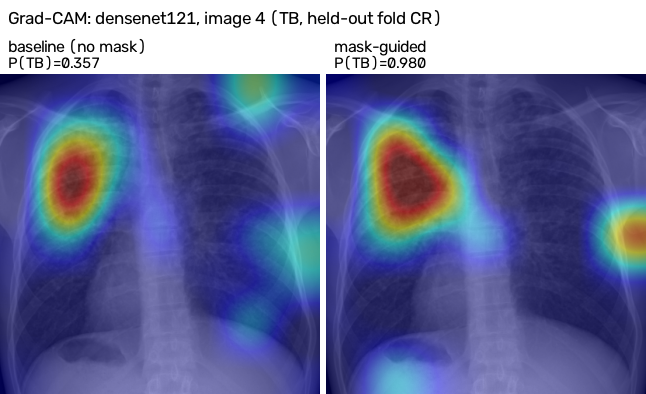
\includegraphics[width=0.85\textwidth]{fig2_mask_guided.png}
\caption{Grad-CAM for DenseNet-121 on the same held-out TB case, baseline
(left) vs.\ mask-guided (right). The mask-guided model keeps the baseline's
left-apex focus and adds a second, correct hotspot on the right, flipping a
misclassification (P(TB)=0.357) to a correct call (P(TB)=0.980).}
\label{fig:maskcam}
\end{figure}

\section{Conclusion}

Our recommended TB/Normal classifier is a single frozen, LoRA-adapted
RAD-DINO on lung-cropped input, trained with strong image-level
augmentation under leave-one-modality-out folds and no batch-level mixup.
It reaches F1@0.5 of 0.9913 internally and 0.8966 / 0.8976 on the external
Shenzhen and Montgomery cohorts, the best external numbers in this line of
work and the first to reach the 89\% Shenzhen accuracy of our earlier
DenseNet-121 baseline [1].

We arrived at it by subtraction. A component-wise ablation showed that
strong augmentation carries essentially all of the domain-generalization
benefit, that domain-aware mixup actively hurts, and that the LOMO split --
which we retain as the honest validation protocol -- is not itself a source
of generalization. Four independent attempts to do better by adding
something (a second foundation model, a mask channel, mask-guided
attention, dual-stream fusion) each improved or held the internal number
while losing external ground.

The methodological point generalizes past this challenge. Across seven DG
configurations and four architectural variants, internal F1 was a poor and
at times inverted guide to external F1: the single best internal
configuration we trained is among the worst on Montgomery. Model selection
for deployable CXR screening has to be done on genuinely external data, and
a paper that reports only a same-source validation number has not yet
reported the thing that matters. A roughly 0.09 F1 internal-to-external gap
remains open; with AUC above 0.96 on both external cohorts, the ranking of
patients survives domain shift far better than the fixed 0.5 threshold
does, which we take as the most promising direction for closing it.

\paragraph{Note on the challenge submission.} The model submitted to the
TREAT-MMTB 2026 challenge was the earlier RAD-DINO + CheXFound ensemble,
selected before the external validation reported here was complete. The
submission stands as a matter of record; the single-backbone configuration
above is what this paper recommends, and the difference between the two is
itself an instance of the paper's argument.

\begin{thebibliography}{15}

\bibitem{ssrn}
[1] Anonymized for review: Domain Generalization of Tuberculosis Detection in
Chest X-Rays through MixStyle and Multi-Level Augmentation. SSRN 5644210.

\bibitem{who2023}
[2] World Health Organization: Global Tuberculosis Report 2023. WHO, Geneva
(2023).

\bibitem{raddino}
[3] P\'erez-Garc\'ia, F., et al.: RAD-DINO: Exploring Scalable Medical Image
Encoders Beyond Text Supervision. arXiv:2401.10815 (2024).

\bibitem{chexfound}
[4] CheXFound: A Chest X-Ray Foundation Model with Global and Local
Representation Integration. (2024/2025).

\bibitem{dinov2}
[5] Oquab, M., et al.: DINOv2: Learning Robust Visual Features without
Supervision. arXiv:2304.07193 (2023).

\bibitem{lora}
[6] Hu, E.J., et al.: LoRA: Low-Rank Adaptation of Large Language Models. ICLR
(2022).

\bibitem{mixstyle}
[7] Zhou, K., Yang, Y., Qiao, Y., Xiang, T.: Domain Generalization with
MixStyle. ICLR (2021).

\bibitem{randconv}
[8] Xu, Z., et al.: Robust and Generalizable Visual Representation Learning via
Random Convolutions. ICLR (2021).

\bibitem{delcom}
[9] Wang, Z., Xia, Y.: Domain-Aware Mixup for Robust Chest X-Ray Diagnosis
Across Unseen Domains. (2022).

\bibitem{densenet}
[10] Huang, G., Liu, Z., van der Maaten, L., Weinberger, K.Q.: Densely Connected
Convolutional Networks. CVPR (2017).

\bibitem{swin}
[11] Liu, Z., et al.: Swin Transformer: Hierarchical Vision Transformer using
Shifted Windows. ICCV (2021).

\bibitem{convnext}
[12] Liu, Z., et al.: A ConvNet for the 2020s. CVPR (2022).

\bibitem{torchxrayvision}
[13] Cohen, J.P., et al.: TorchXRayVision: A library of chest X-ray datasets and
models. MIDL (2022).

\bibitem{jaeger}
[14] Jaeger, S., et al.: Two public chest X-ray datasets for computer-aided
screening of pulmonary diseases. Quant. Imaging Med. Surg. 4(6), 475--477
(2014).

\bibitem{tbx11k}
[15] Liu, Y., Wu, Y.-H., Ban, Y., Wang, H., Cheng, M.-M.: Rethinking
Computer-Aided Tuberculosis Diagnosis. CVPR (2020).

\end{thebibliography}

\end{document}
